 \documentclass{beamer}[10]

\usepackage{graphicx}
\usepackage{xcolor}
\usepackage{tabto}
%\usepackage{beamerthemesplit}
\usepackage{tikz}
\usepackage{cancel}
\usepackage{verbatim}
\usepackage{fancybox}
\usepackage{enumerate}
\usepackage{amsmath,amssymb,amsthm,textcomp,mathtools}
\usepackage[super]{nth}
\usepackage[amssymb]{SIunits}
\usepackage{booktabs}
\usepackage{cancel}
\usepackage{bm}
\usepackage[utf8]{inputenc}
\usepackage{tabularx}
\usepackage{ragged2e}
\newcolumntype{Y}{ >{\RaggedRight\arraybackslash}X}
\usetikzlibrary{arrows,shapes}
\newcommand\T{\rule{0pt}{2.6ex}}
\newcommand\B{\rule[-1.2ex]{0pt}{0pt}}
\definecolor{UUcrimson}{RGB}{204,0,0}
\mode<presentation>
{ \usetheme{default}
  \usecolortheme[named=UUcrimson]{structure}
  \useinnertheme{circles}
  \setbeamercovered{transparent}
  \setbeamertemplate{blocks}[rounded]
  \usefonttheme[onlymath]{serif}
  \setbeamertemplate{navigation symbols}{}
  \setbeamertemplate{footline}[page number]
  \setbeamertemplate{navigation symbols}{}
  \setbeamercolor{section in toc}{fg=black,bg=white}
  \setbeamercolor{alerted text}{fg=UUcrimson!80!gray}
  \setbeamercolor*{palette primary}{fg=white,bg=UUcrimson}
  \setbeamercolor*{palette secondary}{fg=UUcrimson!70!black,bg=gray!15!white}
  \setbeamercolor*{palette tertiary}{bg=UUcrimson!80!black,fg=gray!10!white}
  \setbeamercolor*{palette quaternary}{fg=UUcrimson,bg=gray!5!white}
  \setbeamercolor*{palette sidebar primary}{fg=UUcrimson!10!black}
  \setbeamercolor*{palette sidebar secondary}{fg=white}
  \setbeamercolor*{palette sidebar tertiary}{fg=UUcrimson!50!black}
  \setbeamercolor*{palette sidebar quaternary}{fg=gray!10!white}
  \setbeamercolor{titlelike}{parent=palette primary,fg=white}
  \setbeamercolor{frametitle}{bg=UUcrimson}
  \setbeamercolor{frametitle right}{bg=UUcrimson}
  \setbeamercolor*{separation line}{}
  \setbeamercolor*{fine separation line}{}
}

\usetikzlibrary{backgrounds}
\makeatletter
\tikzstyle{every picture}+=[remember picture]
\tikzset{%
  fancy quotes/.style={
    text width=\fq@width pt,
    align=justify,
    inner sep=1em,
    anchor=north west,
    minimum width=\linewidth,
    font=\itshape
  },
  fancy quotes width/.initial={.8\linewidth},
  fancy quotes marks/.style={
    scale=8,
    text=white,
    inner sep=0pt,
  },
  fancy quotes opening/.style={
    fancy quotes marks,
  },
  fancy quotes closing/.style={
    fancy quotes marks,
  },
  fancy quotes background/.style={
    show background rectangle,
    inner frame xsep=0pt,
    background rectangle/.style={
      fill=gray!25,
      rounded corners,
    },
  }
}
\newenvironment{fancyquotes}[1][]{%
\noindent
\tikzpicture[fancy quotes background]
\node[fancy quotes opening,anchor=north west] (fq@ul) at (0,0) {``};
\tikz@scan@one@point\pgfutil@firstofone(fq@ul.east)
\pgfmathsetmacro{\fq@width}{\linewidth - 2*\pgf@x}
\node[fancy quotes,#1] (fq@txt) at (fq@ul.north west) \bgroup}
{\egroup;
\node[overlay,fancy quotes closing,anchor=east] at (fq@txt.south east) {''};
\endtikzpicture}
\makeatother

\usepackage{scalerel}[2014/03/10]
\usepackage{stackengine}
\usepackage{empheq}
\newcommand*\widefbox[1]{\fbox{\hspace{0.5em}#1\hspace{0.5em}}}

\newcommand\reallywidetilde[1]{\ThisStyle{%
  \setbox0=\hbox{$\SavedStyle#1$}%
  \stackengine{-.1\LMpt}{$\SavedStyle#1$}{%
    \stretchto{\scaleto{\SavedStyle\mkern.2mu\sim}{.5467\wd0}}{.4\ht0}%
%    .2mu is the kern imbalance when clipping white space
%    .5467++++ is \ht/[kerned \wd] aspect ratio for \sim glyph
  }{O}{c}{F}{T}{S}%
}}
\usepackage{media9}

\logo{
\includegraphics[width=0.75cm]{logo.jpg}}
\author[Gibbs]{Dr. Jeremy A. Gibbs}
\institute{Department of Mechanical Engineering\\University of Utah}
\date{Fall 2016}
\title{LES of Turbulent Flows: Lecture 14}

\begin{document}

%----------------------------------------------------------------------------------------
%	TITLE & TOC SLIDES
%----------------------------------------------------------------------------------------

\begin{frame} 
  \titlepage
\end{frame}

%------------------------------------------------

\begin{frame}
\frametitle{Overview}
\tableofcontents
\end{frame}

%------------------------------------------------
\section{Recap: Smagorinsky Model} %
%------------------------------------------------
\begin{frame}{Recap: Eddy-Viscosity Models}
\begin{itemize}
	\item In Lecture 12 we said that eddy-viscosity models are of the form:
	\begin{align*}
		\text{momentum} \qquad \tau_{ij} &= -2\nu_{T} \widetilde{S}_{ij}\\
		\text{scalars} \qquad q_i &= -D_T \frac{\partial \widetilde{\theta}}{\partial x_i}
	\end{align*}
	where
	$$D_T = \frac{\nu_T}{\text{Pr}},$$
	\item $\widetilde{S}_{ij}$ is the filtered strain rate
	\item $\nu_T$ is eddy-viscosity
	\item $D_T$ is eddy-diffusivity
	\item Pr is the SGS Prandtl number 
\end{itemize}

\end{frame}

%------------------------------------------------

\begin{frame}{Recap: Smagorinsky Model}
$$\nu_T = (C_S \Delta)^2 | \widetilde{S}|$$

\begin{itemize}
	\item $\Delta = (\Delta_x \Delta_y \Delta_z)^{\frac{1}{3}}$ is the effective grid scale (see Deardorff 1970 or Scotti et al, 1993)
	\item $C_S \Delta$ is the length scale -- squared for dimensional consistency
	\item $|\widetilde{S}| = \sqrt{2\widetilde{S}_{ij}\widetilde{S}_{ij}}$ is the magnitude of the filtered strain rate tensor with units of [$T^{-1}$]. It serves as part of the velocity scale -- think $\partial \langle u \rangle / \partial z$ in Prandtl's theory
\end{itemize}

\end{frame}

%------------------------------------------------
\begin{frame}{Recap: Smagorinsky Model}

\begin{itemize}
	\item The final model is 
	$$\tau_{ij} - \frac{1}{3}\tau_{kk}\delta_{ij} = -2\nu_{T} \widetilde{S}_{ij} = -2 (C_S \Delta)^2 | \widetilde{S}| \widetilde{S}_{ij}$$
	\item In order to close the model, we need a value of $C_S$ (usually called the Smagorinsky or Smagorinsky-Lilly coefficient)
	\item In Lecture 13 we derived an expression for the Smagorinsky coefficient and showed that $C_S\approx0.17$ (for a spectral cutoff filter)
\end{itemize}

\end{frame}

%------------------------------------------------
\begin{frame}{Recap: Smagorinsky Model}
\begin{itemize}
	\item Recall that dimensionally,
	$$\nu_T = \left[ \frac{L^2}{T}\right] \sim U\ell$$
	\item Smagorinsky model prescribed both $U$ and $\ell$
	\item Subsequent models attempted to improve adaptation of the eddy-viscosity approach to local flow properties
	\item One-equation models prescribe $\ell$, while $U$ is predicted by the flow
	\item In two-equation models, both $\ell$ and $U$ are predicted by the flow
\end{itemize}

\end{frame}

%------------------------------------------------
\section{Two-Equation Eddy-Viscosity Models} %
%------------------------------------------------
\begin{frame}{Two-Equation Eddy-Viscosity Models}
\begin{itemize}
	\item Deardorff (1973): model the evolution of $\tau_{ij}$ (Sagaut pg. 243)
	\begin{align*}
		\frac{\partial \tau_{ij}}{\partial t} &= -\frac{\partial (\bar u_k \tau_{ij})}{\partial x_k}	- \tau_{ik}\frac{\partial \bar u_j}{\partial x_k} - \tau_{jk}\frac{\partial \bar u_i}{\partial x_k}\\
		&\underbrace{-\frac{\partial (\overline{u_i^\prime u_j^\prime u_k^\prime})}{\partial x_k}}_{\text{I}} + \underbrace{p^\prime \left(\overline{\frac{\partial u_i^\prime}{\partial x_j} + \frac{\partial u_j^\prime}{\partial x_i}}\right)}_{\text{II}}\\
		&\underbrace{-\frac{\partial (\overline{u_i^\prime p^\prime})}{\partial x_j}}_{\text{III}} -\underbrace{\frac{\partial (\overline{u_j^\prime p^\prime})}{\partial x_i}}_{\text{IV}} -\underbrace{2\nu\left(\overline{\frac{\partial u_i^\prime}{\partial x_k}\frac{\partial u_j^\prime}{\partial x_k}}\right)}_{\text{V}}
	\end{align*}
	\item where subgrid kinetic energy $k_r = \tau_{kk}/2$
  	\item The terms in this equation have to be modeled.
\end{itemize}

\end{frame}

%------------------------------------------------
\begin{frame}{Two-Equation Eddy-Viscosity Models}
\begin{itemize}
	\item I (tripple correlation)
	$$\overline{u_i^\prime u_j^\prime u_k^\prime} = -C_{3m} f(k_r, \tau_{ij})$$
	\item II (pressure-strain correlation)
	$$p^\prime \left(\overline{\frac{\partial u_i^\prime}{\partial x_j} + \frac{\partial u_j^\prime}{\partial x_i}}\right) = -C_m f(k_r, \tau_{ij})$$
	\item III, IV (pressure-velocity correlations) were ignored
	\item V (dissipation)
	$$2\nu\left(\overline{\frac{\partial u_i^\prime}{\partial x_k}\frac{\partial u_j^\prime}{\partial x_k}}\right) = C_e f(k_r)$$
	\item where $C_m = 4.13$, $C_e=0.7$, and $C_{3m}=0.2$
  
\end{itemize}

\end{frame}

%------------------------------------------------
\begin{frame}{Two-Equation Eddy-Viscosity Models}
\begin{itemize}
	\item To close the model, a separate equation for subgrid turbulence kinetic energy ($k_r$) is required.
	\item This model is similar to the a \nth{2}-order RANS closure (see Speziale 1991 for a review of RANS closures including \nth{2}-order models) 
	\item The need for these additional equations add significantly to the complexity and computational cost of the simulation
	\item Despite the added complexity, the models are still subject to the limitations of the basic eddy-viscosity approach
\end{itemize}

\end{frame}

%------------------------------------------------
\section{One-Equation Eddy-Viscosity Models} %
%------------------------------------------------
\begin{frame}{One-Equation Eddy-Viscosity Models}
\begin{itemize}
	\item Deardorff (1980) suggested a simpler 1-equation approach to avoid the need  to solve prognostic equations for $\tau_{ij}$ (in addition to N-S equations) 
	\item This model is equivalent to a $k$-$\ell$ 1-equation RANS model (see Speziale, 1991)
	\item This was also proposed earlier for the isotropic part of a 2-part eddy-viscosity model by Schumann (1975).
\end{itemize}

\end{frame}

%------------------------------------------------

\begin{frame}{One-Equation Eddy-Viscosity Models}
\begin{itemize}
	\item However, the model is usually credited to Deardorff (especially in the atmospheric community)
	\item Models based on D80 are popular in the atmospheric boundary layer due to the ability to include SGS transport or energy drain effects as extra parameters in the SGS TKE equation (\textit{e.g.} for SGS canopy drag,  buoyancy forces, etc.)  
\end{itemize}

\end{frame}

%------------------------------------------------
\begin{frame}{One-Equation Eddy-Viscosity Models}
\begin{itemize}
	\item In this model, $\ell$ is prescribed and $U$ is predicted by the flow
	\item Assume that $U\sim \sqrt{k_r}$
	\item Thus, eddy-viscosity is modeled as
	$$\nu_T = C_1\ell_d\sqrt{k_r}$$
	\item Here, $C_1(\sim0.1)$ is the ``Deardorff coefficient''
	\item $C_1 \ell_d$ is $\ell$ (similar to Smagorinsky) and $\sqrt{k_r}$ is $U$
	\item Thus, the model is given by
	$$\tau_{ij} = -2 C_1\ell_d\sqrt{k_r}\widetilde{S}_{ij}$$
	\item In order to close this model, we must prescribe $\ell_d$ and determine $k_r$ from a separate transport equation.
\end{itemize}

\end{frame}

%------------------------------------------------
\begin{frame}{One-Equation Eddy-Viscosity Models}
\begin{itemize}
	\item The parameterized dimensional form of the $k_r$ transport equation according to D80 is given by:
	$$\frac{\partial k_r}{\partial t} = - \frac{\partial \tilde{u}_j k_r}{\partial x_j} + 2 \nu_T S_{ij}S_{ij} - D_T \frac{\partial \tilde{b}}{\partial z} \nonumber + \frac{\partial}{\partial x_j}2 \nu_T \frac{\partial k_r}{\partial x_j} - \epsilon$$
	where, $\tilde{b} = (g/\theta_o)\tilde{\theta}$ is buoyancy, $\theta_o$ is a constant reference potential temperature, and $\tilde{\theta}$ is potential temperature
	\item To complete this transport equation and close the model, we need expressions for $\nu_T$, $D_T$, and $\epsilon$
\end{itemize}

\end{frame}

%------------------------------------------------
\begin{frame}{One-Equation Eddy-Viscosity Models}
\begin{itemize}
	\item According to D80
	\begin{align*}
		\nu_T &= C_1\ell_d\sqrt{k_r}	\\
		D_T &= \left( 1 + 2\frac{\ell_d}{\Delta} \right)\nu_T \\
		\epsilon &= C_e \frac{k_r^{3/2}}{\ell_d}
	\end{align*}
	where$$C_e = f_c \left(0.19+0.51 \cfrac{\ell_d}{\Delta}\right)$$
	and$$f_c = 1 + \frac{2}{\left(\cfrac{z_w}{\Delta z_w} + 1.5\right)^2 - 3.3}$$

\end{itemize}

\end{frame}

%------------------------------------------------

\begin{frame}{One-Equation Eddy-Viscosity Models}
\begin{itemize}
	\item A note from D80 about $f_c$, which is used to enhance near-wall dissipation (in our notation):
	\begin{fancyquotes}
		Close to the surface, however, $C_e$ was increased by a `wall-effect' factor of up to 3.9 to prevent $k_r$ from becoming unduly large there
	\end{fancyquotes}
	\item Some later studies (\textit{e.g.} Moeng 1984) merely set $C_e = 3.9$ at the first model level.
	\item Others follow that of Nieuwstadt (1990) by using $f_c$
	\item Your instructor believes the latter is more physically meaningful and in the spirit of Deardorff's comment.
\end{itemize}
\end{frame}
%------------------------------------------------

\begin{frame}{One-Equation Eddy-Viscosity Models}
\begin{itemize}
	\item Finally, we have to prescribe $\ell_d$
	\begin{gather*}
	\ell_d = 
	\begin{cases}
	\Delta & \cfrac{\partial \tilde{b}}{\partial z} \leq 0\\\\
	\mathrm{min}\left[\Delta,\cfrac{1}{2}\cfrac{\sqrt{k_r}}{N}\right]  & \cfrac{\partial \tilde{b}}{\partial z} > 0
	\end{cases}
	\end{gather*}
	where $N = \sqrt{\partial \tilde{b}/{\partial z}}$ is the Brunt-V\"{a}is\"{a}l\"{a} frequency 
	\item D80 tied the notion of the grid scale to static stability (\textit{i.e.}, as static stability increases, the characteristic length scale should reduce to less than the effective grid spacing)
\end{itemize}
\end{frame}

%------------------------------------------------

\begin{frame}{One-Equation Eddy-Viscosity Models}
\begin{itemize}
	\item The complete D80 model in dimensional form:
	\begin{align*}
	\tau_{ij} &= -2 C_1\ell_d\sqrt{k_r}\widetilde{S}_{ij}\\
	\frac{\partial k_r}{\partial t} &= - \frac{\partial \tilde{u}_j k_r}{\partial x_j} + 2 \nu_T S_{ij}S_{ij} - D_T \frac{\partial \tilde{b}}{\partial z} \nonumber + \frac{\partial}{\partial x_j}2 \nu_T \frac{\partial k_r}{\partial x_j} - \epsilon\\
	\nu_T &= C_1\ell_d\sqrt{k_r}	\\
		D_T &= \left( 1 + 2\frac{\ell_d}{\Delta} \right)\nu_T \\
		\epsilon &= C_e \frac{k_r^{3/2}}{\ell_d}\\
		\ell_d &= \Delta (\partial \tilde{b}/\partial x_3 \leq 0), \mathrm{min}\left[\Delta,0.5\sqrt{k_r}/N\right] (\partial \tilde{b}/\partial x_3 > 0)
	\end{align*}

\end{itemize}

\end{frame}

%------------------------------------------------

\begin{frame}{One-Equation Eddy-Viscosity Models}
\begin{itemize}
	\item Another form of the transport equation is given in dimensionless form (see Geurts pg 227, Debliquy 2001)
	$$\frac{\partial k_r}{\partial t} = - \frac{\partial \tilde u_j k_r}{\partial x_j} + \frac{\partial}{\partial x_j}\left(\frac{C_2}{C_1} \Delta \sqrt{k_r}\frac{\partial k_r}{\partial x_j}\right) + \frac{1}{\text{Re}}\frac{\partial^2 k_r}{\partial x_j^2} + \Pi - \epsilon$$
	\item viscous dissipation is typically modeled based on isotropy assumption $\epsilon = (C_k/\Delta)k_r^{3/2}$
	\item $C_2$ is a constant on the order of unity and $C_k\approx1.7$ is the Kolmogorov ``constant''
	\item Note: the transport terms for pressure and SGS kinetic energy have been modeled by the \nth{2}-term on the RHS of the equation
\end{itemize}

\end{frame}

%------------------------------------------------

\begin{frame}{One-Equation Eddy-Viscosity Models}
Gibbs and Fedorovich (2016) addressed issues w/ D80
\begin{itemize}
	\item Does the closure require the stability-dependent turbulence length-scale?
	\item The Prandtl number formulation can lead to stability patchiness
	\item Is there a need for near-wall enhancement of dissipation anymore?
\end{itemize}

\end{frame}

%------------------------------------------------

\begin{frame}{One-Equation Eddy-Viscosity Models}
\begin{itemize}
	\item To address the first point, GF16 eliminates the stability dependence of the length scale assuming that the grid spacing is small enough to match, at least approximately, the reduced turbulence length-scale?
	$$\ell_d = \Delta$$
\end{itemize}

\end{frame}

%------------------------------------------------

\begin{frame}{One-Equation Eddy-Viscosity Models}
\begin{itemize}
	\item To address the second point, GF16 creates a new formulation of the Prandtl number ($\text{Pr}=\nu_T/D_T$)
	\item Using the D80 formulations
	$$\text{Pr} = \left(1 + 2\frac{\ell_d}{\Delta}\right)^{{-1}}$$
	which means based on the stability criteria
	\begin{gather*}
\text{Pr} = 
\begin{cases}
1/3 & \frac{\partial \tilde{b}}{\partial z} \leq 0\\
\rightarrow 1 \mbox{ as } \ell_d \rightarrow 0  & \frac{\partial \tilde{b}}{\partial z} > 0
\end{cases}
\end{gather*}
\item This means that under stable conditions, with $\ell_d < \Delta$, $\nu_T$ is persistently smaller than $D_T$, while most studies (\textit{e.g.}, Ohya 2001, Grachev et al. 2007, Zilitinkevich et al. 2012) show that at least with moderate stability Pr$\approx1$.
\end{itemize}

\end{frame}

%------------------------------------------------

\begin{frame}{One-Equation Eddy-Viscosity Models}
\begin{itemize}
	\item In addition, GF16 reported that the use of the D80 approach sometimes led to problematic patchiness of the resolved fields when adjoining cells were of opposite stability.
	\item The new formulation is:
	\begin{gather*}
\text{Pr} = 
\begin{cases}
\left(3 - 2e^{-\mathrm{Ri}^2}\right)^{-1} & \frac{\partial \tilde{b}}{\partial z} \leq 0\\
1  & \frac{\partial \tilde{b}}{\partial z} > 0
\end{cases}
\label{prnew}
\end{gather*}
where $\mathrm{Ri}$ is the gradient Richardson number
$$\mathrm{Ri} = \frac{\cfrac{\partial \tilde{b}}{\partial z}}{ \Bigg(\cfrac{\partial \tilde{u}}{\partial z}\Bigg)^2 +\Bigg(\cfrac{\partial \tilde{v}}{\partial z}\Bigg)^2}$$
\end{itemize}

\end{frame}

%------------------------------------------------

\begin{frame}{One-Equation Eddy-Viscosity Models}
  
\setlength{\fboxsep}{0pt}
\setlength{\fboxrule}{1pt}
\begin{columns}[T]
    \begin{column}{.45\textwidth}
    \begin{itemize}
    	\item $C_1$ is D80, $C_2$ is GF16
    	\item The outcome is that the relative effect of mechanical mixing is enhanced with stable stratification compared to the original formulation of D80
    \end{itemize}
    \end{column}
    \begin{column}{.55\textwidth}
    \begin{minipage}[c][.6\textheight][c]{\linewidth}
      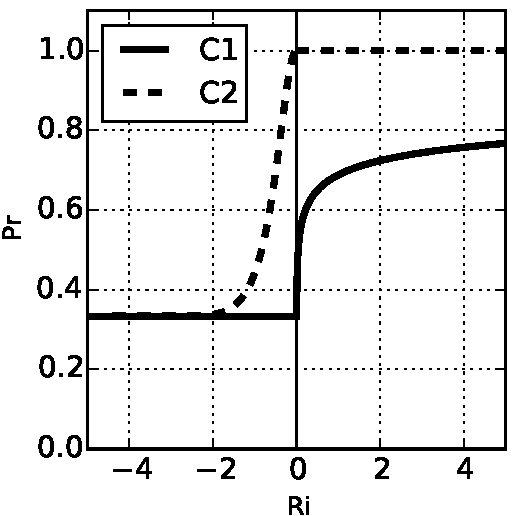
\includegraphics[width=\textwidth]{prandtl.pdf}
      \end{minipage}
    \end{column}
  \end{columns}
  
\end{frame}

%------------------------------------------------

\begin{frame}{One-Equation Eddy-Viscosity Models}
  
\setlength{\fboxsep}{0pt}
\setlength{\fboxrule}{1pt}
\begin{columns}[T]
    \begin{column}{.45\textwidth}
    \begin{itemize}
    	\item Finally, GF16 suggests that near-wall enhancement of dissipation is unnecessary, provided that the grid spacing is adequately small.
	\item This argument follows the findings in Moeng et al (2007), which effectively corresponds to setting $f_c=1$
    \end{itemize}
    \end{column}
    \begin{column}{.55\textwidth}
    \begin{minipage}[c][.6\textheight][c]{\linewidth}
      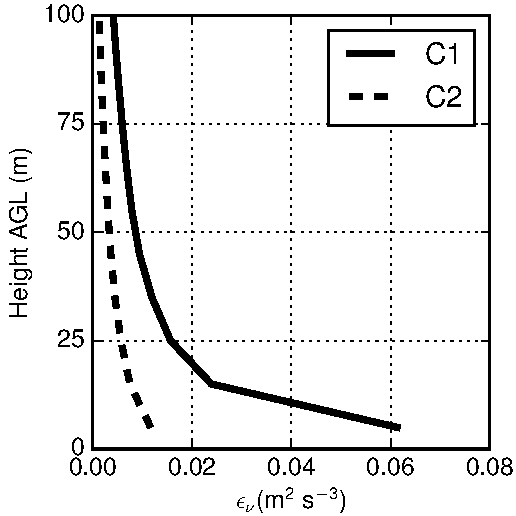
\includegraphics[width=\textwidth]{dissipation.pdf}
      \end{minipage}
    \end{column}
  \end{columns}
  
\end{frame}

%------------------------------------------------

\begin{frame}{One-Equation Eddy-Viscosity Models}
\begin{itemize}
	\item The GF16 modifications to D80 are summarized here
	\begin{align*}
\nu_T &=C_1 \Delta \sqrt{k_r} \mbox{ ,} \\
D_T &= 
\begin{cases}
\left(3 - 2e^{-\mathrm{Ri}^2}\right)\nu_T & \frac{\partial \tilde{b}}{\partial z} \leq 0\\
\nu_T  & \frac{\partial \tilde{b}}{\partial z} > 0
\end{cases},\\
\epsilon &= 0.7 \frac{E^{\frac{3}{2}}}{\Delta} \mbox{ .}
\end{align*}
\end{itemize}

\end{frame}

%------------------------------------------------

\begin{frame}{One-Equation Eddy-Viscosity Models}
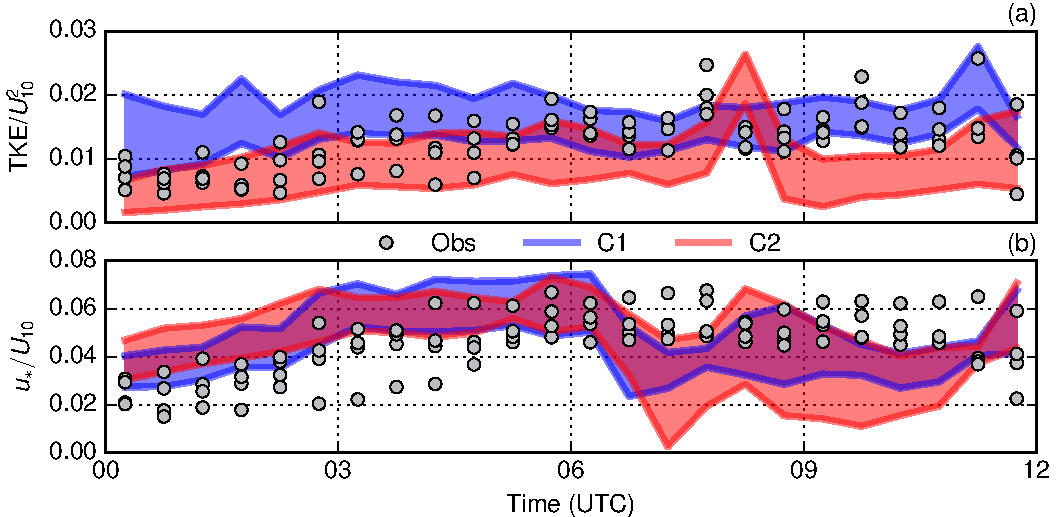
\includegraphics[width=\textwidth]{Gibbs_Fig7.pdf}
\begin{itemize}
	\item New formulation seems to better capture near-surface TKE until flow becomes really stable ($t\approx8\hour$)
	\item Both formulations seem to overpredict $u_*$ under moderate stability and overpredict when the flow becomes more stable. 
\end{itemize}

\end{frame}

%------------------------------------------------

\begin{frame}{One-Equation Eddy-Viscosity Models}
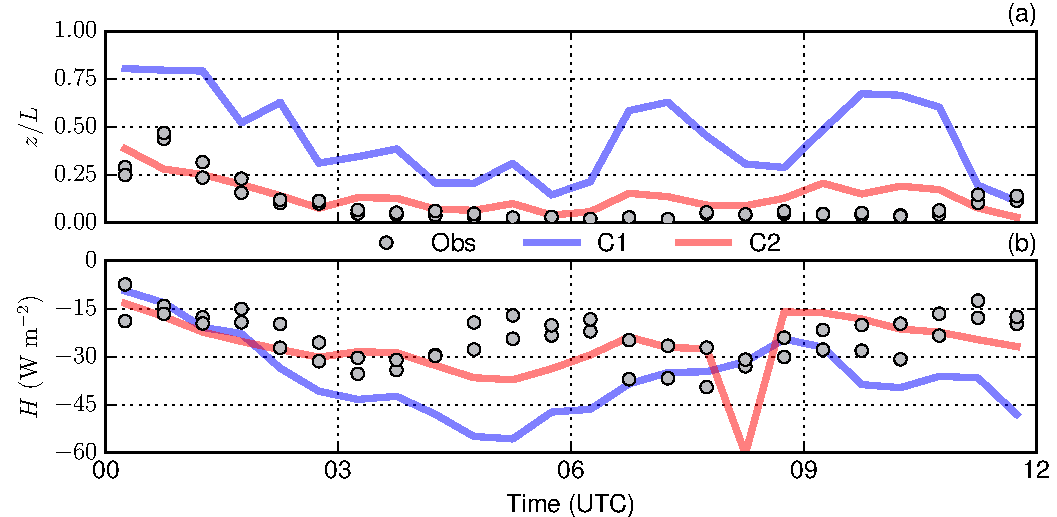
\includegraphics[width=\textwidth]{Gibbs_Fig8.pdf}
\begin{itemize}
	\item New formulation seems to better capture near-surface stability of the flow
	\item New formulation seems to better capture the near-surface sensible heat flux
\end{itemize}

\end{frame}

%------------------------------------------------

\begin{frame}{One-Equation Eddy-Viscosity Models}
Gibbs and Fedorovich (2016) has weak points
\begin{itemize}
	\item Run for a single case
	\item Grid spacing of $10\ \metre$ might be too coarse to meet the assumptions of the modifications
	\item The LES code used was driven (initialized and nudged in time) by a large-scale weather model (WRF), which means the formulations may be sensitive to model bias
	\item The LES code uses low-order advection schemes
\end{itemize}

\end{frame}

%------------------------------------------------
\section{Two-Point Eddy-Viscosity Models} %
%------------------------------------------------
\begin{frame}{Two-Point Eddy-Viscosity Models}
\begin{itemize}
	\item Based on Metais and Lesieur, 1992
	\item See Sagaut pg 124 or Lesieur et al., 2005 ``Large-Eddy Simulation of Turbulence''
	\item This model is an attempt to go beyond the Smagorinsky model while keeping, in physical space, the same scaling as the spectral eddy-viscosity model of Kriachnan (1976) 
\end{itemize}

\end{frame}
%------------------------------------------------
\begin{frame}{Two-Point Eddy-Viscosity Models}
\begin{itemize}
	\item Idea: in physical space build an eddy-viscosity normalized by
	$$\sqrt{\frac{E_{\vec{x}}(k_c)}{k_c}} \qquad \text{with} \qquad k_c = \frac{\pi}{\Delta}$$
	and where $E_{\vec{x}}$ is the local kinetic energy spectrum at point $\vec{x}$
\end{itemize}

\end{frame}

%------------------------------------------------
\begin{frame}{Two-Point Eddy-Viscosity Models}
\begin{itemize}
	\item $E_{\vec{x}}$ must be evaluated in terms of physical space quantities.  The best candidate for this is the \nth{2}-order structure function:
	$$F^{\text{iso}} (r) = \left\langle \left[ \vec{u}(\vec{x},t) - \vec{u}(\vec{x}+\vec{r},t)\right]^2\right\rangle$$
	\item Note: the isotropic \nth{2}-order structure function spectrum (Fourier transform) is  equivalent to the the Kolmogorov $k^{-5/3}$ energy spectrum
	\item See Pope sections 6.2 and 6.4, Wyngaard (2010), Gibbs and Fedorovich (2016b) for the relationship between structure functions and energy spectrum
\end{itemize}

\end{frame}

%------------------------------------------------
\begin{frame}{Two-Point Eddy-Viscosity Models}
\begin{itemize}
	\item For the two-point eddy-viscosity model, the local structure function is used
	$$F_2(\vec{x},\Delta) = \left\langle \left[ \widetilde{\vec{u}}(\vec{x},t) - \widetilde{\vec{u}}(\vec{x}+\vec{r},t)\right]^2\right\rangle_{||\vec{r}||}$$
	where we now have a local statistical average over the nearest 6 points (or 4 points in a boundary layer).
	\item Assuming a $k^{-5/3}$ energy spectrum from 0 to $k_c$, we get
	$$\boxed{\nu_T(\vec{x}, \Delta, t) = 0.0105 C_k^{-3/2} \Delta \sqrt{F_2(\vec{x}, \Delta)}}$$
	where $C_k$ is the Kolmogorov ''constant''
\end{itemize}

\end{frame}

%------------------------------------------------
\begin{frame}{Two-Point Eddy-Viscosity Models}
\begin{itemize}
	\item If we replace the velocity increments by \nth{1}-order spatial derivatives, we can show that 
	$$\nu_T \approx 0.777 (C_S\Delta)^2 \sqrt{2\widetilde{S}_{ij}\widetilde{S}_{ij} - \tilde{\omega_i}\tilde{\omega_i}}$$
	where $\tilde{\omega} = \vec{\nabla} \times \widetilde{\vec{u}}$ is the filtered vorticity.
	\item We can imagine that the two-point (or structure function) model is the Smagorinsky model in a strain/vorticity formulation 
\end{itemize}

\end{frame}

%------------------------------------------------

\end{document}

